\chapter{Results}
In this chapter our results are presented. Starting off with a description f the graph database, we then move on to the three different cases. 

\section{Graph Database}
% Power of graph databases
We are dealing with connected data, where choosing a graph database have two advantages according to \citet{robinson2013}: performance and flexibility. In a relational database, the join-intensive query performance deteriorates as the dataset gets larger while, with a graph database the performance remains relatively constant. This is due to the fact that a query is only localized to a fraction of the graph making the run time proportional to the size of the sub-graph related to the query rather than the overall graph containing all available data.

Furthermore, there is the aspect of flexibility. Graphs are naturally additive \cite{robinson2013} such that new sub-graphs can be added containing more nodes and edges and new relations can be introduced as the understanding of the dataset grows. This have a positive implication for the analysts that does not have to model the domain in exhaustive detail from the start but can add information as time progress. 

Thus, according to the motivation above, we expect to use Neo4j, which is a cloud based graph database supporting some basic analysis through their query language Cypher.

\section{Gh0st RAT Controllers}

The result for the RAT controller case is given in table \ref{aucIndex}. The table shows the AUC values and the F$_1$ score for the different indices (as rows) and different numbers of reference nodes, that the similarity is based on. Since cross validation is performed, 20 trials has been performed. We find small variance in the results.

\begin{table}[h!]
    \centering
    \caption{AUC for different number of reference nodes. The AUC is calculated from the precision-recall curve. The F$_1$ score represents the highest accuracy for in each run.}
    \begin{tabular}{|c||c|c||c|c||c|c||c|c||c|c|}
      \hline
      \multirow{2}{*}{~} 
            & \multicolumn{2}{c||}{1}
            & \multicolumn{2}{c||}{2}
            & \multicolumn{2}{c||}{3}
            & \multicolumn{2}{c||}{4}
            & \multicolumn{2}{|c|}{5} \\             \cline{2-11}
      ~     &AUC&F$_1$&AUC&F$_1$&AUC&F$_1$&AUC&F$_1$&AUC&F$_1$ \\ \hline
    Dice    &0.8995 & 0.89 & 0.9363 &0.94 &0.9554&0.97 & 0.9627 &0.98&0.9658 & 0.98 \\
    Jaccard &0.8978 & 0.89 & 0.9367 &0.94 &0.9552&0.97 & 0.9616 &0.98&0.9654 & 0.98 \\
    Cosine  &0.8943 & 0.89 & 0.9337 &0.94 &0.9518&0.97 & 0.9591 &0.98&0.9621 & 0.98 \\
    ProHub  &0.8850 & 0.89 & 0.9244 &0.94 &0.9435&0.97 & 0.9478 &0.98&0.9434 & 0.98 \\
    DeHub   &0.8987 & 0.89 & 0.9378 &0.94 &0.9563&0.97 & 0.9631 &0.98&0.9664 & 0.98 \\
    LP      & 0.7930 & 0.78 & 0.9283 & 0.96 & 0.9279 & 0.96 & 0.9426 & 0.98 & 0.9206 & 0.98 \\ 
    Katz    & 0.1888 & 0.29 & 0.1960 & 0.28 & 0.1949 & 0.26 & 0.1759 & 0.28 & 0.1850 & 0.27 \\ \hline
    \end{tabular}
    \label{aucIndex}
\end{table}


With all the described indices and the mentioned parameters, all RAT controllers were identified properly, with a precision of 100\% and a recall of 100\%.

Futhermore, there were three IP addresses that were constantly 

% In how many of the cases did we classify the three IP addresses as RAT controllers?
    
The second data set was much more sparse of RAT controllers. Of 10091 nodes, only 32 were identified as RAT controllers. Performing the exact same analysis on this data set as the previous one gave us the result shown in table \ref{aucIndex2}.

\begin{table}[h!]
    \centering
    \caption{AUC for different number of reference nodes. The AUC is calculated from the precision-recall curve.}
    \begin{tabular}{|c||c|c||c|c||c|c||c|c||c|c|}
      \hline
      \multirow{2}{*}{~} 
            & \multicolumn{2}{c||}{1}
            & \multicolumn{2}{c||}{2}
            & \multicolumn{2}{c||}{3}
            & \multicolumn{2}{c||}{4}
            & \multicolumn{2}{|c|}{5} \\             \cline{2-11}
      ~     &AUC&F$_1$&AUC&F$_1$&AUC&F$_1$&AUC&F$_1$&AUC&F$_1$ \\ \hline
    Dice    & 0.9696 & 0.98 & 0.9680 & 1.00 & 0.9531 & 1.00 & 0.9375 & 1.00 & 0.9219 & 1.00 \\
    Jaccard & 0.9696 & 0.98 & 0.9680 & 1.00 & 0.9531 & 1.00 & 0.9375 & 1.00 & 0.9219 & 1.00 \\
    Cosine  & 0.9696 & 0.98 & 0.9680 & 1.00 & 0.9531 & 1.00 & 0.9375 & 1.00 & 0.9219 & 1.00 \\
    ProHub  & 0.9696 & 0.98 & 0.9680 & 1.00 & 0.9531 & 1.00 & 0.9375 & 1.00 & 0.9297 & 1.00 \\
    DeHub   & 0.9696 & 0.98 & 0.9680 & 1.00 & 0.9531 & 1.00 & 0.9375 & 1.00 & 0.9219 & 1.00 \\ 
    LP      & 0.7930 & 0.78 & 0.9283 & 0.96 & 0.9279 & 0.96 & 0.9426 & 0.98 & 0.9206 & 0.98 \\ 
    Katz    & 0.1888 & 0.29 & 0.1960 & 0.28 & 0.1949 & 0.26 & 0.1759 & 0.28 & 0.1850 & 0.27 \\ \hline
    \end{tabular}
    \label{aucIndex2}
\end{table}




\section{Classification of malicious IP addresses}

The best accuracy was found for the parameters $C=100$ and $\gamma=1$. These values were then used throughout the classification. 

The results are presented in table \ref{IpRes}. The table presents the average over 100 trials and the standard deviation with a confidential level of 95 \%. The SVM classifier, based on all 6 input features, performed prediction with an accuracy of 50 \%. Futhermore, ... of the predicted classes were higher than Recorded Future's while ... \% were lower. 

\begin{table}[h!]
    \centering
    \caption{Results from the SVM classifier using six features. The table shows the fraction of correct predictions (accuracy), the fraction of higher predictions and the fraction of lower predictions in relation to Recorded Future's actual classification.}
    \begin{tabular}{|c|c|c|}
    \hline
        ~   & Mean & Std  \\ \hline
        Correct predictions & 0.9952 &  0.9903 \\
        Higher predictions  & 0.9952 &  0.9903\\
        Lower predictions   & 0.9952 &  0.9903\\ \hline
    \end{tabular}
    \label{IpRes}
\end{table}

The results from including only the two topological features are presented in table \ref{IpRes2Feat}. The features were PageRank and degree of the node. The table presents the average over 100 trials and the standard deviation with a confidential level of 95 \%. The SVM classifier performed prediction with an accuracy of 50 \%. Futhermore, ... of the predicted classes were higher than Recorded Future's while ... \% were lower. 

\begin{table}[h!]
    \centering
    \caption{Results from the SVM classifier using two features. The table shows the fraction of correct predictions (accuracy), the fraction of higher predictions and the fraction of lower predictions in relation to Recorded Future's actual classification.}
    \begin{tabular}{|c|c|c|}
    \hline
        ~   & Mean & Std  \\ \hline
        Correct predictions & 0.9952 &  0.9903 \\
        Higher predictions  & 0.9952 &  0.9903\\
        Lower predictions   & 0.9952 &  0.9903\\ \hline
    \end{tabular}
    \label{IpRes2Feat}
\end{table}

The results from including only four features are presented in table \ref{IpRes4Feat}. The features included information about the number of hits and the neighbours co-occurrence with malwares, cyber vulnerabilities and attack vectors. The table presents the average over 100 trials and the standard deviation with a confidential level of 95 \%. The SVM classifier performed prediction with an accuracy of 50 \%. Futhermore, ... of the predicted classes were higher than Recorded Future's while ... \% were lower. 

\begin{table}[h!]
    \centering
    \caption{Results from the SVM classifier using four features. The table shows the fraction of correct predictions (accuracy), the fraction of higher predictions and the fraction of lower predictions in relation to Recorded Future's actual classification.}
    \begin{tabular}{|c|c|c|}
    \hline
        ~   & Mean & Std  \\ \hline
        Correct predictions & 0.9952 &  0.9903 \\
        Higher predictions  & 0.9952 &  0.9903\\
        Lower predictions   & 0.9952 &  0.9903\\ \hline
    \end{tabular}
    \label{IpRes4Feat}
\end{table}

For a pseudorandom classifier, the results can be found in table \ref{randClass}.

\begin{table}[h!]
    \centering
    \caption{Results from the a pseudorandom classifier. The table shows the fraction of correct predictions (accuracy), the fraction of higher predictions and the fraction of lower predictions in relation to Recorded Future's actual classification.}
    \begin{tabular}{|c|c|c|}
    \hline
        ~   & Mean & Std  \\ \hline
        Correct predictions & 0.9952 &  0.9903 \\
        Higher predictions  & 0.9952 &  0.9903\\
        Lower predictions   & 0.9952 &  0.9903\\ \hline
    \end{tabular}
    \label{randClass}
\end{table}

\section{Prediction of Future Cyber Attacks}
The AUC and prediction rate of predicting future cyber attacks using PLP on the data set described in \secref{cyberattacks} is shown in \figref{fig:plp_auc} for different lengths of the set used for testing.
\begin{figure}[!ht]
\centering
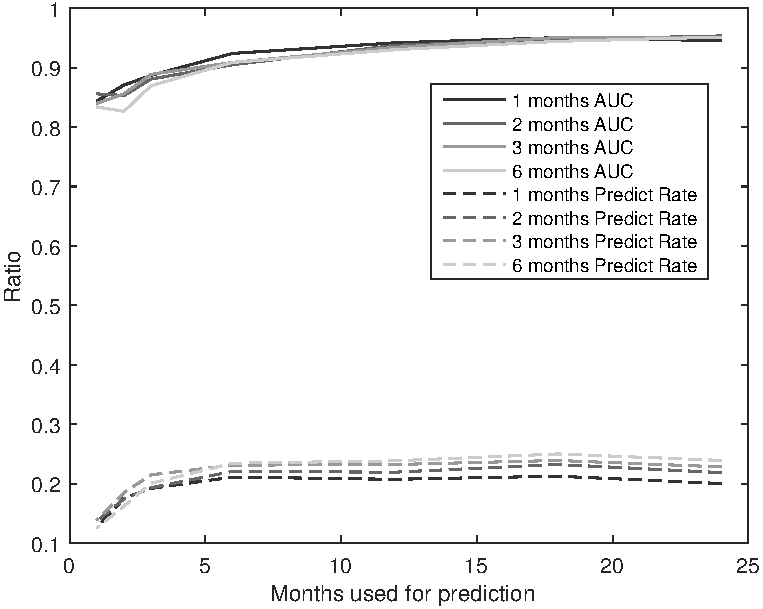
\includegraphics[scale=0.9]{images/auc_plp_result.pdf}
\caption{\label{fig:plp_auc} AUC and Prediction rate for the PLP algorithm used on the cyber attack bipartite graph. The different shades of grays represent differents length of time period used for testing (in months). AUC was calculated according to the description in section \ref{plp:auc} and prediction rate according to \ref{plp:predict_rate}.}
\end{figure}

How great the natural limitations of the algorithm are can be seen in \figref{fig:plp_max} where the maximum possible prediction rate, the ratio of cyber attacks with same actors as was previously seen in the prediction set and the ratio of cyber attacks that involved at least one new actor is presented.

\begin{figure}[!ht]
\centering
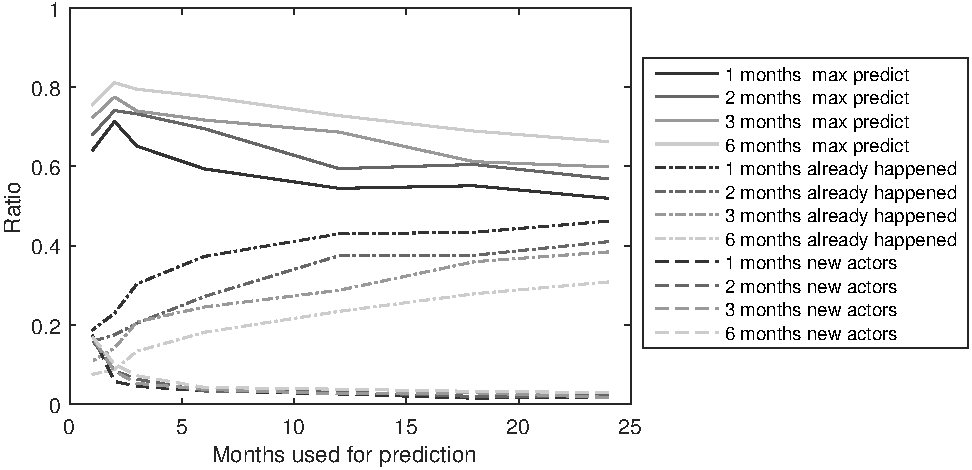
\includegraphics[width=\textwidth]{images/max_plp_result.pdf}
\caption{\label{fig:plp_max} 
Maximum prediction rate possbile for PLP for comarison with the prediction rate in \figref{fig:plp_auc}. Also showing the ratio of attacks with set of actors already in prediction set as well as the ratio of attacks involving at least one new actor.}
\end{figure}

We find that the auc increases around 10 percent units from 1 month of prediction data to 24 months of prediction data. However, the prediction rate does not vary that much for length of prediction data of at least 6 months.

